\section{Infrastruttura di rete}
\subsection{Descrizione}
L'infrastruttura di rete dell'azienda Rius.Co. comprende ben due reti diverse: la rete aziendale, della quale fanno parte le sottoreti degli uffici amministrativi, operativi e di segreteria, e la rete dei server che comprende i 4 server sulla quale è costruito il Marketplace. La rete aziendale sarà per l'appunto interna all'azienda e quindi locale. La rete dei server sarà invece esterna in quanto collocata all'interno di una rete VPC (Virtual Private Cloud) disponibile tramite il Google Cloud \cite{VPC}. 
\medskip

L'affitto di reti VPC è uno dei tanti servizi che offre Google per ospitare server e applicazioni web, in particolare questo servizio consiste nella creazione di una rete basata su la topologia virtuale fornita dagli utenti. Ho scelto questo servizio in quanto in passato avevo già avuto esperienze pratiche con la piattaforma cloud di Google; proprio grazie ai corsi online offerti dal programma Qwiklabs ho acquistato familiarità con le reti VPC e tutti i dispositivi che ne fanno parte \cite{Qwiklabs}. Google inoltre fornisce una grande quantità di strumenti che permettono ai programmatori di concentrarsi più sui servizi che stanno sviluppando che sull'infrastruttura che li circonda. Un esempio importante è la tecnologia HA Cloud VPN che permette di collegare tramite un tunnel VPN ad alta affidabilità (99.99\% garantito) la rete locale di un'azienda alle reti VPC collocate sul cloud \cite{CloudVPN}. La tecnologia Cloud VPN si basa sul protocollo IPSec ed implementa una Secure VPN di tipo site-to-site che non richiede una complessa configurazione manuale dell'utente. Le reti VPC fanno parte del nuovo approccio alle architetture di rete chiamato Software-defined networking (SDN) \cite{SDN}, si basano quindi sulla virtualizzazione delle reti e se ne guadagna perciò in termini di affidabilità, scalabilità, flessibilità e riduzione dei costi.
\medskip

Attraverso l'HA Cloud VPN i dipendenti dell'azienda potranno quindi collegarsi da remoto alla rete VPC che contiene i server, la sede aziendale sarà quindi collegata ad Internet tramite un ISP e il traffico dei dipendenti collegati dall'azienda passerà per un Firewall che filtrerà i messaggi in entrata ed uscita. Nella sede aziendale saranno presenti un Campus Distributor che si interfaccerà con la rete pubblica dell'ISP per ottenere l'accesso ad Internet, sarà poi presente un Building Distributor in quanto si prevede la presenza di un solo edificio e infine ci saranno due Floor Distributor, uno per il piano che ospiterà la segreteria e l'ufficio operativo e un altro per il piano che ospiterà l'ufficio amministrativo. I collegamenti saranno costruiti con cavi ethernet di categoria 6A con schermatura completa SFTP che garantiscono un buon bandwidth (circa 10Gbps su 100 metri), forte stabilità grazie alla doppia schermatura e un risparmio considerevole visto il prezzo di circa 1 euro al metro \cite{Cables}. Questo tipo di collegamento risulta quindi perfetto per i dispositivi che faranno parte della rete: router, switch, PC fissi e stampanti. 
\subsection{Apparati di rete}
All'interno della sede aziendale saranno presenti un numero contenuto di apparati di rete fisici in quanto la parte più importante ed esposta dell'infrastruttura è contenuta nella rete VPC. I seguenti apparati di rete fisici costituiranno la rete dell'azienda: 
\begin{itemize}
    \item \textbf{Router esterno con Firewall}, si occupa di ricevere la connessione dal Campus Distributor e filtrare i messaggi implementando delle rigide politiche tramite le access list definite dall'amministratore di rete. I messaggi ritenuti validi verranno inoltrati al router interno che si occuperà di recapitarli alla destinazione;
    \item \textbf{Router interno con DHCP}, si occupa dell'instradare i pacchetti all'interno della rete aziendale e di assegnare automaticamente gli indirizzi IP ai dispositivi. Ho scelto di non includere un server DHCP per ragioni economiche e di manutenzione, l'azienda non dispone di numerose postazioni perciò un semplice router è in grado di gestire l'instradamento dei pacchetti e il servizio DHCP senza grossi problemi;
    \item \textbf{Switch}, ho scelto di includere tre switch con ventiquattro porte ciascuno in vista di futuri aggiornamenti della rete o l'acquisizione di ulteriore personale. 
\end{itemize}
Ho scelto di non inserire un server email in quanto comporta una spesa importante per l'azienda che però non ottiene in cambio vantaggi consistenti ma anzi si trova a dover condurre una manutenzione costante del server, i servizi online di email in questo caso si dimostrano più economici e adatti al contesto dell'azienda. Infine, non ho incluso nessun access point in quanto per poter offrire la copertura totale di un edificio di due piani la spesa che dovrebbe sostenere l'azienda sarebbe ingiustificabile, in questo caso è quindi preferibile non disporre di connettività wireless ma concentrare le spese sullo sviluppo di un'infrastruttura robusta ed espandibile. 
\subsection{Server}
L'infrastruttura prevede l'implementazione di ben 4 diversi tipi di server divisi su 3 strati o tier, ogni strato è in grado di comunicare esclusivamente con lo strato direttamente superiore o inferiore al proprio. Questa architettura è considerata ottimale in quanto rispetta i principi di scalabilità verticale ed orizzontale delle applicazioni, è inoltre alla base dei sistemi distribuiti con interfaccia web. L'architettura a 3 tier è particolarmente adatta per l'ambiente web in quanto è molto comune avere diversi componenti slegati tra loro che concorrono e cooperano per il funzionamento della web app \cite{3Tier}. 
\medskip

Il primo strato è chiamato Presentation Layer e comprende sia il Web server che l'API server, questo è l'unico strato in cui i server sono esposti all'esterno e raggiungibili direttamente attraverso il proprio indirizzo IP. Gli utenti quando richiedono una pagina web o fanno una richiesta tramite l'API interagiscono direttamente con questo strato che si occupa di eseguire una prima elaborazione di queste richieste prima di inoltrare i dati al livello sottostante. Sono presenti entrambi i server in questo strato in quanto entrambi si occupano di rispondere alle richieste di client che sono però di tipo diverso. L'API server è stato inserito anche per rendere più facile il futuro sviluppo dell'applicazione mobile che potrebbe essere sviluppata come un semplice front-end che dialoga con l'API tramite le richieste HTTPS. 
\medskip

Subito dopo troviamo invece l'Application Layer, questo contiene l'application server nel quale sono presenti tutti i programmi e i processi che rappresentano e rispettano la logica dell'applicazione o sito web. Le funzioni appartenenti all'Application Layer vengono invocate direttamente dal Presentation Layer che invia anche i dati necessari per completare l'elaborazione delle richieste degli utenti. Questo è forse lo strato più importante perché senza di esso il resto sarebbe totalmente inutile in quanto non conterrebbe nulla della logica con la quale è stata pensata la web app. 
\medskip

Abbiamo infine lo Storage Layer che comprende il data server, quest'ultimo conserva e gestisce l'accesso a tutti i dati relativi al programma e salvati all'interno di database o cartelle locali. Nel caso di Rius.Co. oltre al database il data server contiene anche le immagini di profilo degli utenti e quelle legate ai prodotti. In questo strato viene condotta un ulteriore rifinitura dei dati per accertarsi che gli utenti non stiano provando a danneggiare l'infrastruttura attraverso attacchi come l'SQL injection. 

\begin{figure}[ht]
    \centering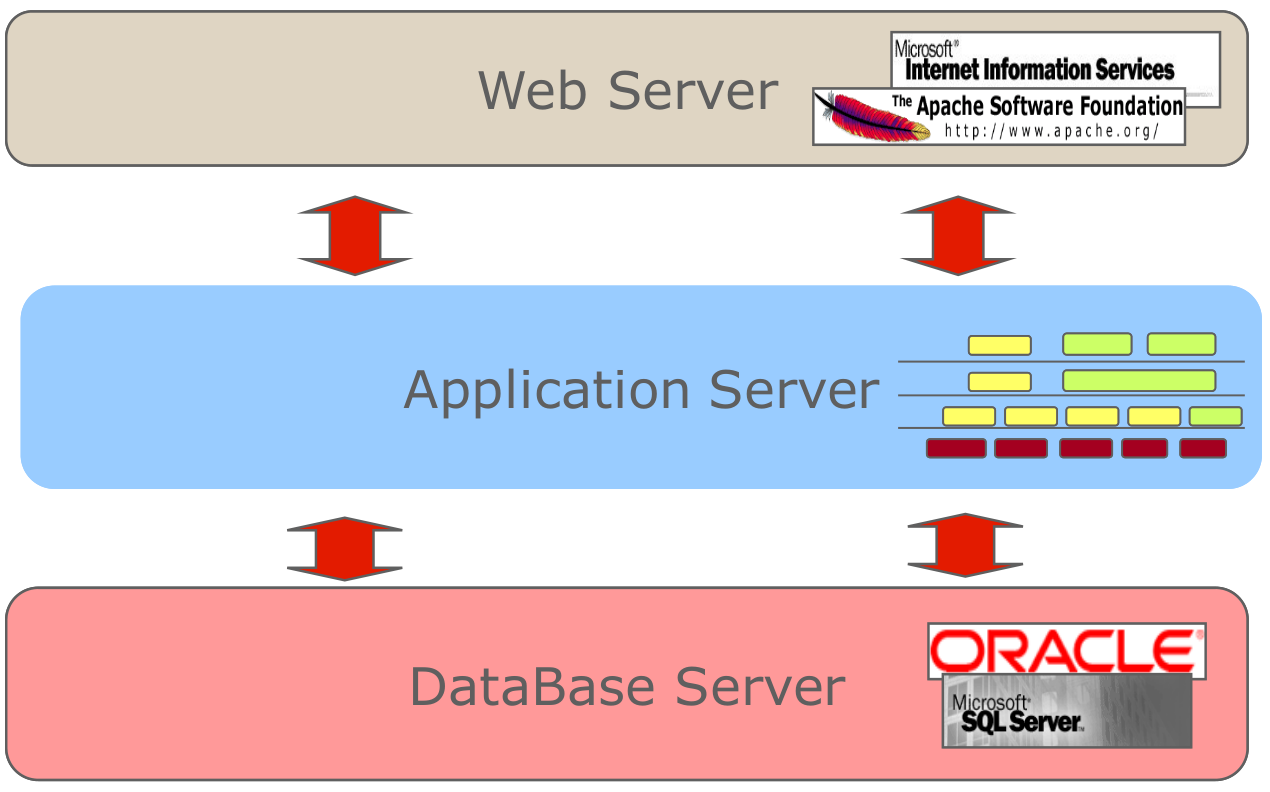
\includegraphics[scale=0.25]{images/3tier.png}
    \caption{Rappresentazione grafica dell'architettura a 3 tier}
\end{figure}

Questi server non esistono fisicamente all'interno dell'infrastruttura in quanto sono delle macchine virtuali generate tramite il Google Kubernetes Engine e collocate all'interno della rete VPC, ciò offre numerosi vantaggi in quanto è possibile affidare alla piattaforma Google la scalabilità delle risorse, la manutenzione dei server e la gestione dei dati. Il Google Kubernetes Engine consiste in un servizio a metà tra l'Iaas (Infrastructure-as-a-Service) e il Paas (Platform-as-a-Service) attraverso il quale gli utenti possono creare dei cluster di container Docker all'interno dei quali viene eseguito del codice creato dagli sviluppatori \cite{Kubernetes}. Questi container di fatto lavorano come delle macchine virtuali ma garantiscono maggiore virtualizzazione e quindi più efficienza e versatilità. Tramite il Google Kubernetes Engine è possibile creare dei cluster di container identici (stesso sistema operativo e hardware) che vengono replicati a seconda del workload globale e dei criteri impostati dall'amministratore. È anche possibile inserire dei Load Balancer che si occupino di dividere equamente la mole di lavoro all'interno dei cluster di macchine virtuali, insieme a questi è consigliato integrare anche degli Health Checks che in caso di disservizi eseguono azioni predefinite come l'invio istantaneo di un email di notifica all'amministratore. 
\subsection{Progetto di rete} 
Ho progettato la rete aziendale includendo anche la rete VPC usando il programma di simulazione Cisco Packet Tracer 8.0, nelle etichette da me inserite sono riportati gli indirizzi IP degni di nota e le informazioni relative alle 4 sottoreti create. Il file è stato caricato assieme a tutto il progetto nell'apposita repository creata su GitHub e \href{https://github.com/MauroPello/elaborato}{raggiungibile qui} \cite{GitHub}. 
\begin{figure}[ht]
    \centering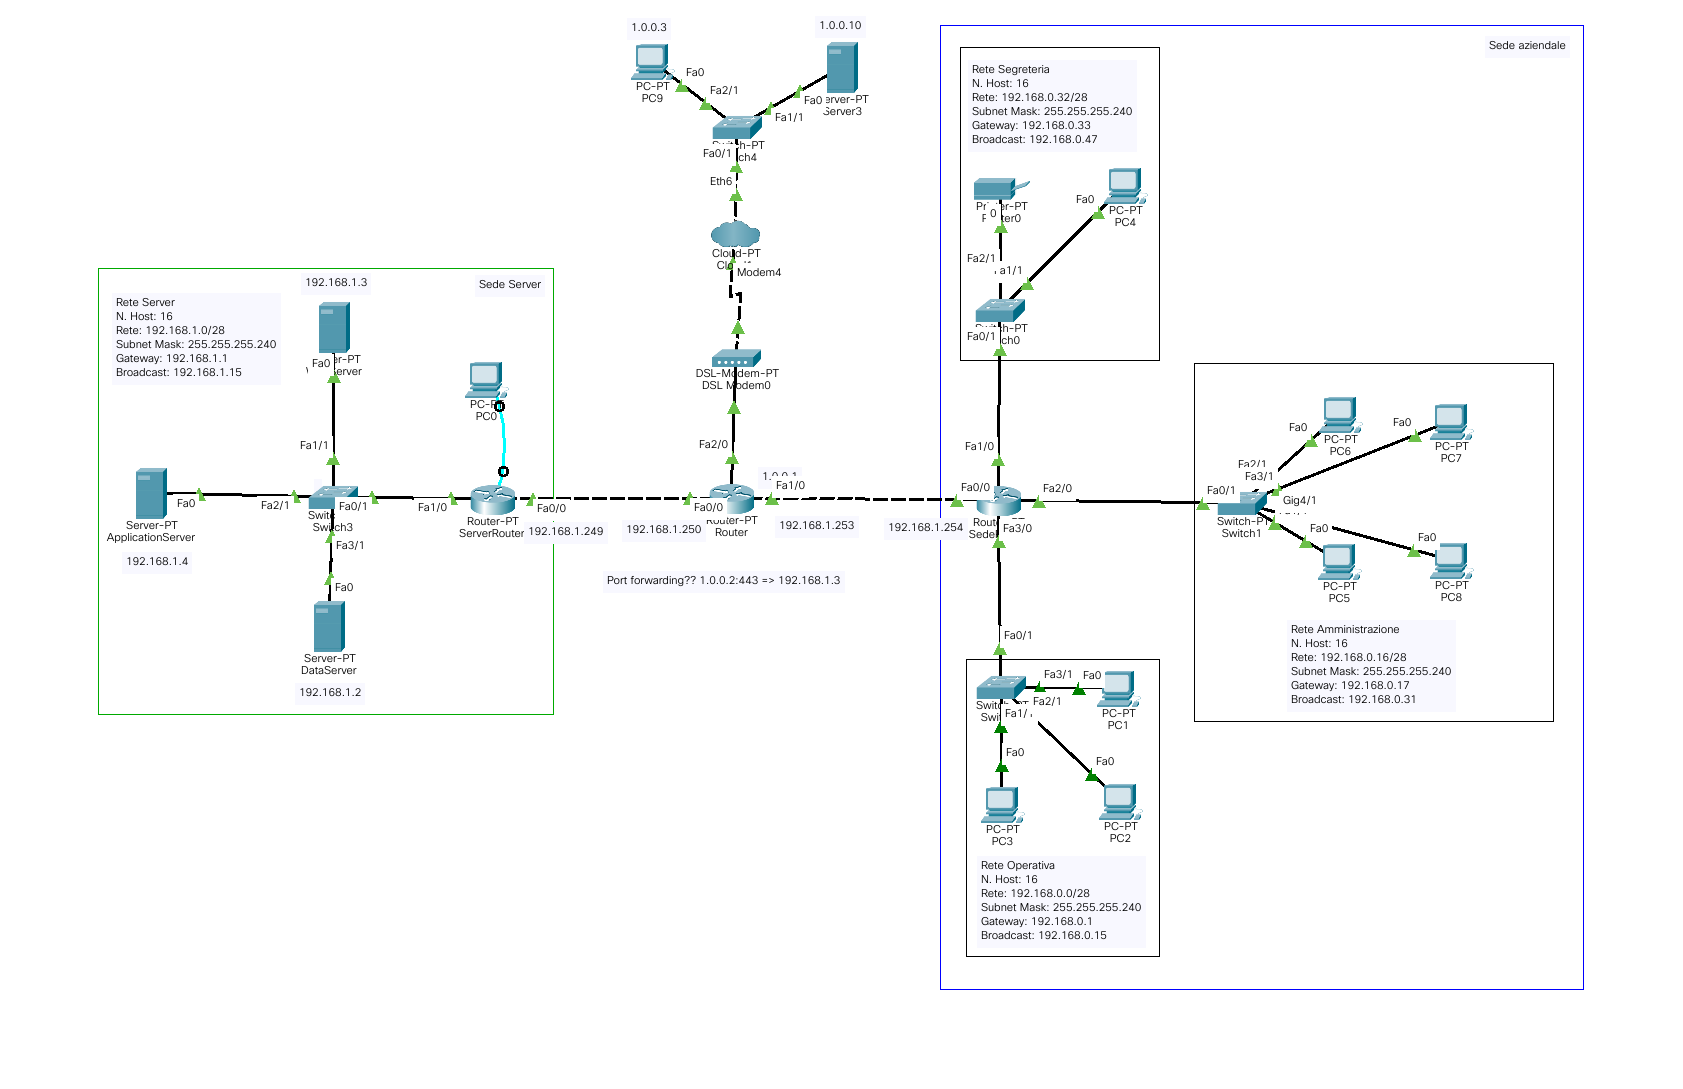
\includegraphics[scale=.51]{images/rete.png}
\end{figure}